% File acl2014.tex

\documentclass[11pt]{article}
\usepackage{acl2014}
\usepackage{multirow}
\usepackage{times}
\usepackage[tone]{tipa}
\usepackage{url}
\usepackage{latexsym}
\usepackage{phonetic}
\usepackage{graphicx}

%\setlength\titlebox{5cm}

% You can expand the titlebox if you need extra space
% to show all the authors. Please do not make the titlebox
% smaller than 5cm (the original size); we will check this
% in the camera-ready version and ask you to change it back.

\title{The effects of lexical phonotactics, saturation,
  and frequency skew on segmentability}
%
%\author{Benjamin B{\"o}rschinger \\
%    Macquarie University\\
%    Heidelberg University \And
%    Robert Daland \\
%    Linguistics \\
%    UCLA \And
%    Abdellah Fourtassi \\
%    LCSP \\
%    ENS/EHESS/CNRS \And
%    Emmanuel Dupoux \\
%    LCSP \\
%    ENS/EHESS/CNRS\AND
%    {\tt benjamin.borschinger@mq.edu.au}\\
%    {\tt \{r.daland$\mid$abdellah.fourtassi$\mid$emmanuel.dupoux\}@gmail.com}}

\date{}

\begin{document}
\maketitle
\begin{abstract}
  Previous works have proposed that the `segmentability' of a language
  depends on its phonotactic structure and can be measured as the
  entropy of licit segmentations of a corpus sample. These proposals
  are tested here by generating artificial languages and measuring
  their segmentability. Maximally permissive and restrictive grammars
  (Pseudo-Berber, Pseudo-Senufo) were used to generate corpus samples 
  in which the lexical saturation and frequency distributions were
  varied parametrically. The results show heretofore  unsuspected
  nuances of the relationship between phonotactic complexity, word
  length, and word segmentation.
\end{abstract}


\section{Introduction}
\vspace*{-5pt}
Word segmentation is the perceptual process by which infant and adult listeners parse the continuous speech signal into a sequence of discrete, word-like units. The acquisition of word segmentation has been the subject of intense computational scrutiny, where it is typically operationalized as the unsupervised partitioning of a phonemically transcribed, child-directed corpus, and assessed against an orthographically derived gold standard~\cite{Goldwater09a,Daland11a,Pearl10b}.

A number of modeling studies indicates that across a typologically diverse range of languages (e.g. Arabic, Japanese, Korean, Russian, and Spanish), and across a range of models (lexical, phonotactic, and hybrid), better segmentation is unfailingly found for English than for other languages \cite{Fleck08a,Daland09a,Daland11a,Fourtassi13a,Daland13a}. The empirical data bearing on this point is sparse, and occasionally conflicting \cite{Nazzi06a,Nazzi14a}. Therefore, while current models may be insufficient, it seems worth considering the possibility that languages genuinely differ with respect to how easy they are to segment. Along those lines, Daland and Zuraw~\shortcite{Daland13a} investigated the segmentability of Korean using a phonotactic segmentation model~\cite{Daland11a}, finding that Korean's many edge-sensitive phonological processes did not help word segmentation. Fourtassi et al.~\shortcite{Fourtassi13a} compared the segmentability of Japanese and English using lexical segmentation models~\cite{Goldwater09a,Johnson09a} and argued that the comparatively poor segmentability of Japanese was strongly predicted by the `normalized segmentation entropy' of a corpus, the average (per-character) entropy over all licit segmentations of a corpus given the gold standard lexicon. Both Daland and Zuraw and Fourtassi et al. speculated that the poor segmentability of these languages bears close connection to their restrictive phonotactics. The present study seeks to test this proposal by applying a popular Bayesian word segmentation model~\cite{Brent99a,Goldwater07c,Goldwater09a} to artificially generated corpora. Artificial corpora are used here for the same reason that psycholinguistic experiments use carefully controlled stimuli: the complexity of natural language corpora depends on complex and potentially not understood relationships between interacting language properties. For example, it stands to reason that the word frequency distribution might differ between, e.g., Japanese and English for essentially syntactic (and morphological) reasons. By generating artificial corpora, it is possible to vary one property (phonotactics, frequency distributions, word lengths) while holding other factors constant, controlling (to a certain extent) the impact of these additional factors. In fact, this is exactly what the present paper does.

\section{Methods}
\vspace*{-5pt}
Two artificial grammars were created, representing extremes of phonotactic permissiveness and restrictiveness. Pseudo-Senufo is a strict CV grammar -- words must begin with a consonant and end with a vowel.
Pseudo-Berber has no phonotactic constraints whatsoever -- every possible sequence of consonants and vowels is grammatical. Artificial lexicons were generated for each grammar as a sample from the space of phonotactically licit forms; average word length was manipulated using a gradient penalty (see below). From a generated lexicon, a corpus was generated by imposing a word frequency distribution. The word frequency distribution can be manipulated (see below); thus, this generation dissociates phonotactic properties from word frequency distribution properties.
 
\subsection{Generating lexicons from phonotactic grammars}

A \textit{phonotactic grammar} assigns a probability distribution over possible lexical items ($\mu:~\Sigma^* \rightarrow[0,1]$). The alphabet $\Sigma$ used here is a small but standard segmental inventory: [ptk|fsx|mn\textipa{N}|lr|wj|aeiou]. Phonotactic grammars were defined using the maximum entropy harmonic grammar framework~\cite{Hayes08a}: `features' are constraints penalizing particular dimensions of ill-formedness (e.g. the constraint \textsc{Onset} penalizes words which begin with a vowel). Each constraint is associated with a weight, and the `harmony' of a string is the weighted sum of its constraint violations. The log-odds of two forms is the difference in their harmonies, which is sufficient to determine a log-linear model. Thus, a collection of constraints and their weights serves to define a phonotactic grammar. A \textit{lexicon} is generated as a sample (without replacement) from the probability distribution defined by a phonotactic grammar, i.e. a list of $n$ distinct word types. For tractability, a hard maximum string length of 6 was imposed on lexical forms. The Pseudo-Senufo grammar included 4 constraints favoring a CV syllable structure (\textsc{Onset, *Coda, *Hiatus, *Complex}). These constraints were given a sufficiently high weight (-25) as to categorically enforce a CV structure in sample lexicons. It also includes a constraint, \textsc{*Struct}, which penalizes words according to their length, gradiently favoring shorter words. The weight of \textsc{*Struct} was manipulated, yielding varying degrees of pressure for Pseudo-Senufo grammars to `saturate' the space of phonotactically licit short forms. The Pseudo-Berber grammar included only \textsc{*Struct}, allowing any sequence of segments as a licit word-form (`phoneme salad'). 

\subsection{Generating a corpus from a lexicon}

The distribution of patterns in their input plays a crucial role for the outcome of learning for statistical models. Side-stepping the complex interactions between semantics, syntax and morphology that give rise to word distributions in real languages we generate artificial corpora mimicking, to varying degrees, the token distribution of natural language. As a blue-print, we take the type and token statistics from the Brent-Bernstein-Ratner corpus~\cite{Brent99a}, containing a specific distribution for 1365 distinct types and 33347 tokens. From this, we can generate artificial corpora that match this distribution by first sampling 1365 distinct types from the phonotactic grammars described above and then generating a random permutation of 33347 tokens that match the original distribution perfectly.\footnote{To generate utterance boundaries, we assume a stopping probability of $\frac{1}{3}$, resulting in corpora with identical numbers of types and tokens but slightly differing numbers of utterances.} We refer to corpora that follow this distribution as \textsc{bbr}, and also experiment with a distribution in which all types occur with (roughly) the same frequency (\textsc{flat}) to see in how far the frequency distribution has an impact on segmentability.%\footnote{In addition to the \textsc{BBR} and \textsc{FLAT} distributions, we considered a simulated generation based on Zipf's Law; the results were quantitatively similar to \textsc{bbr} and are omitted for reasons of space.}

\subsection{Unigram word segmentation}

The Bayesian model for word segmentation we use is a generative model for sequences of words, built on the non-parametric Dirichlet Process (DP) prior. For reasons of space, we refer the reader to Goldwater~\shortcite{Goldwater07c} for details, providing only a brief explanation. The goal of applying the model to unsegmented input is to identify a segmentation that is compatible with a compact probabilistic lexicon, assigning most of the probability mass to a small number of reusable words. The model assumes a pre-specified prior distribution over admissible words, and here we follow previous work~\cite{Brent99a,Goldwater07c} in using a simple lexical generator: it assigns geometrically decaying probabilities to arbitrary sequences of any length and allows any segment to occur anywhere in a word with equal probability. We deliberately opt for such a na\"{i}ve prior to focus on the information conveyed by the input, rather than any linguistically motivated prior biases learners might bring to the task. Crucially, the DP prior favors lexicons that exhibit a Zipfian rich-get-richer dynamic with relatively few high-frequency items and a long tail of low-frequency items, penalizing degenerate solutions in which every utterance counts as its own word-type. Also, the model assumes that words within an utterance are independent, hence it can be seen as a Unigram language model over the infinite space of admissible words. The goal of learning on this view is identifying the finite number of words that provide a compact explanation of the unsegmented input. While the Unigram assumption has been shown to result in undersegmentation of frequent collocations, we chose this model for its simplicity and because the questions of this paper are by and large independent of this known shortcoming. In particular, our artificial languages fit the Unigram assumption by construction, allowing us to focus on phonotactics and word-frequency related issues.

\section{Results}
\vspace*{-5pt}
Our experimental paradigm follows closely that of Johnson and Goldwater~\shortcite{Johnson09a}. For each of our artificial corpora we run four independent Markov Chains for 1000 iterations using the Adaptor Grammar software~\cite{Johnson07c}, using hyper-parameter sampling and calculating a single marginal maximum a posteriori segmentation for each utterance from the samples collected across all 4 chains during the last 200 iterations. We evaluate segmentation accuracy by calculating the token f-score according to the gold boundaries in the artificial corpora. Token f-score is the harmonic mean of token precision, i.e. the fraction of correctly identified tokens in the posited segmentation over all posited tokens, and token recall, i.e. the fraction of correctly recovered tokens over all tokens in the gold standard. 

The results are given in Figure~\ref{Results.}. Overall, pseudo-Berber seems to be segmented better than pseudo-Senufo, with its best token f-scores for \textsc{bbr} being 95\% compared to 87\% for pseudo-Senufo. In the unnatural \textsc{flat} condition, pseudo-Senufo peaks with 97\%, with pseudo-Berber also reaching 94\%. There also is a clear impact of the \textsc{*Struct} constraint that governs the average word lengths, although the importance of this constraint varies considerably. For \textsc{bbr}, pseudo-Senufo yields a token f-score of 80\%+x for all values of \textsc{*Struct} whereas pseudo-Berber drops to 59\% for \textsc{*Struct}=-5 (i.e., small average word length) but yields a considerably higher token f-score than pseudo-Senufo for \textsc{*Struct} $>$-4. In contrast, \textsc{flat} yields the overall best token f-scores for both pseudo-Berber and pseudo-Senufo for small average word lengths and performs worse for larger average word lengths.


\begin{figure*}[t!]
\begin{minipage}[t]{0.50\paperwidth}%
\vspace{-50pt}
	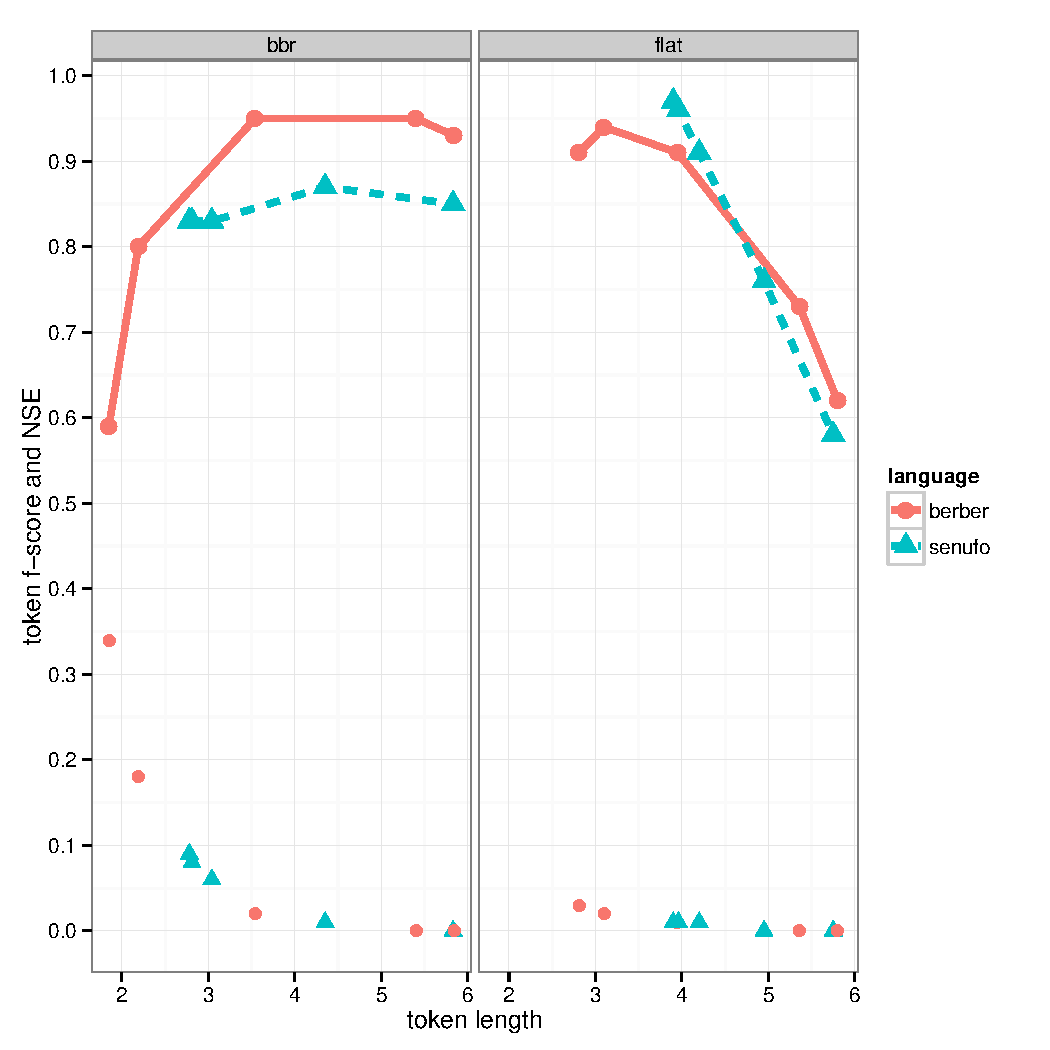
\includegraphics[scale=0.55]{plots/bens_version_2.pdf}
\end{minipage}%
\begin{minipage}[t][1\totalheight][c]{0.3\paperwidth}%
\vspace{0pt}
\scalebox{1.0}{
\begin{tabular}{c|c|c||c}
\textsc{*Struct} &  & berber & senufo\tabularnewline
\hline 
\hline 
\multirow{2}{*}{-1} & SAT & 0.00 & 0.01\tabularnewline
\cline{2-4} 
 & LA & 0.00 & 0.03\tabularnewline
\hline 
\hline 
\multirow{2}{*}{-2} & SAT & 0.00 & 0.33\tabularnewline
\cline{2-4} 
 & LA & 0.05 & 1.03\tabularnewline
\hline 
\hline 
\multirow{2}{*}{-3} & SAT & 0.36 & 0.88\tabularnewline
\cline{2-4} 
 & LA & 1.59 & 0.99\tabularnewline
\hline 
\hline 
\multirow{2}{*}{-4} & SAT & 0.90 & 0.98\tabularnewline
\cline{2-4} 
 & LA & 1.77 & 0.96\tabularnewline
\hline 
\hline 
\multirow{2}{*}{-5} & SAT & 0.99 & 1.00\tabularnewline
\cline{2-4} 
 & LA & 1.75 & 0.95\tabularnewline
\end{tabular}}
\end{minipage}
\caption{\label{Results.} On the left, token f-score (lines) and normalized segmentation entropy (dots) for the different settings, plotted against average token-length. The table lists lexicon ambiguity (LA) and saturation (SAT) for pseudo-Berber and pseudo-Senufo , grouped by \textsc{*Struct}. Small absolute values of \textsc{*Struct} in the table correspond to large average token-length in the figure, and large absolute values to short average token-length.}
\end{figure*}

%
%
%\begin{table*}[t!]
%\begin{center}
%\scalebox{0.9}{
%\begin{tabular}{|c|c|c|c||c|c|c||c|c|c||c|c|c|}
%\cline{5-13} 
%\multicolumn{1}{c}{} & \multicolumn{1}{c}{} & \multicolumn{1}{c}{} & \multicolumn{1}{c|}{} & \multicolumn{3}{c||}{\textsc{brb}} & \multicolumn{3}{c||}{\textsc{zipf}} & \multicolumn{3}{c|}{\textsc{flat}}\tabularnewline
%\hline 
%S & L & LA & SAT & TF & NSE & TL & TF & NSE & TL & TF & NSE & TL\tabularnewline
%\hline 
%\hline 
%\multirow{2}{*}{1} & s & .03 & 0.01 & .85  & .0 & 5.83 & .83  & .0 & 5.87 & .58  & .0 & 5.75\tabularnewline
%\cline{2-13} 
% & b & .0 & 0.00 & .93 & .0 & 5.84 & .91 & .0 & 5.86 & .62  & .0 & 5.80\tabularnewline
%\hline 
%\hline 
%\multirow{2}{*}{2} & s & 1.03 & 0.33 & .87 & .01 & 4.35 & .83 & .0 & 4.94 & .76 & .0 & 4.95\tabularnewline
%\cline{2-13} 
% & b & .05 & 0.00 & \textbf{.95} & .0 & 5.40 & \textbf{.92} & .0 & 5.48 & .73 & .0 & 5.36\tabularnewline
%\hline 
%\hline 
%\multirow{2}{*}{3} & s & .99 & 0.88 & .83 & .06 & 3.04 & .71 & .04 & 3.21 & .91 & .01 & 4.20\tabularnewline
%\cline{2-13} 
% & b & 1.59 & 0.36 & \textbf{.95} & .02 & 3.54 & .87 & .03 & 2.97 & .91 & .01 & 3.95\tabularnewline
%\hline 
%\hline 
%\multirow{2}{*}{4} & s & .96 & 0.98 & .83 & .08 & 2.81 & .68 & .08 & 2.62 & .96 & .01 & 3.96\tabularnewline
%\cline{2-13} 
% & b & 1.77 & 0.90 & .80 & .18 & 2.19 & .62 & .24 & 1.96 & .94 & .02 & 3.10\tabularnewline
%\hline 
%\hline 
%\multirow{2}{*}{5} & s & .95 & 1.00 & .83 & .09 & 2.78 & .67 & .08 & 2.60 & \textbf{.97}  & .01 & 3.90\tabularnewline
%\cline{2-13} 
% & b & 1.75 & 0.99 & .59  & .34 & 1.85 & .45 & .39 & 1.67 & .91  & .03 & 2.81\tabularnewline
%\hline
%\end{tabular}
%}
%\end{center}
%\vspace*{-5pt}
%\caption{\label{Results.}Experimental results, grouped by different values of the \textsc{*Struct} constraint (S column) and language (L column, with ``s'' for pseudo-Senufo and ``b'' for pseudo-Berber). ``TF'' stands for token f-score, ``SE'' for normalized segmentation entropy and ``TL'' for the average gold token length for that condition. We also report lexical saturation (SAT) and lexicon ambiguity (LA) for each experimental setting.}	
%\end{table*}

\section{Discussion}
\vspace*{-5pt}
The results raise several questions. First, it is surprising that the phonotactically much less constrained pseudo-Berber is, on average, more easy to segment, yielding considerably higher token f-scores for the natural  condition than pseudo-Senufo except for \textsc{*Struct}=-5. Even if the segmentation model does not explicitly consider phonotactic cues, a natural expectation would have been that regular phonotactics yield a more regular pattern of lexical forms that would make identification of repeating units easier. There is also considerable variability of segmentability as a function of the frequency distribution and the average word length, with the overall best segmentability achieved for a highly unnatural flat distribution with predominantly short words. This is especially curious, given that the flat distribution violates the model's prior expectation about word frequencies much more strongly than the natural one.

The first observation lends itself to an explanation along the lines of Fourtassi et al.~\shortcite{Fourtassi13a}: we calculate the normalized segmentation entropy (NSE) for the artificial corpora, a measure of how much ambiguity with respect to word segmentation remains if the gold lexicon is provided to the learner, 0 indicating no uncertainty at all and 1.0 indicating complete uncertainty; we refer the reader to \cite{Fourtassi13a} for a more detailed explanation. For \textsc{bbr}, NSE provides a satisfying explanation for the variation in segmentability. Note that for pseudo-Berber, NSE tends to be lower than for pseudo-Senufo for \textsc{*Struct}-values down to roughly -3, and these are exactly the conditions where pseudo-Berber attains higher token f-scores. The trend reverses for \textsc{*Struct}$<$-3, again as would be predicted by looking at NSE. In sum, NSE and token f-score are highly correlated (Person's $r = -0.93$). To understand why NSE varies the way it does, note that for any given word-length, there are strictly less possible word types for pseudo-Senufo than for pseudo-Berber. For example, at the length of 2, there are 65 CV licit sequences for pseudo-Senufo, while there are $18^2$ licit XX sequences for pseudo-Berber. Even in the absence of strong penalties on word length, it will in general be necessary for Pseudo-Senufo to recycle shorter words as sub-parts of longer words.  This picture reverses, however, if the use of long words is heavily penalized. For \textsc{*Struct}$<$-3, pseudo-Berber is effectively limited to words of length 3 to 4 phonemes because longer sequences are penalized so strongly. Now, the absence of any constraint on possible word-forms turns into a disadvantage, due to the high probability of high-frequency single-segment ``words''. Single-segment words cause high segmentation ambiguity because they might be segmented out (incorrectly) whenever the segment occurs. This issue is ameliorated in pseudo-Senufo, where the phonotactic requirements categorically disallow single-segment words. This is clear for \textsc{*Struct}=-4 and \textsc{*Struct}=-5: pseudo-Senufo shows only an increase in NSE from 0.08 to 0.09, while pseudo-Berber's NSE changes from 0.18 to 0.34, and this huge increase in ambiguity is directly reflected in the low token f-score of 59\%, compared to 83\% for pseudo-Senufo. This difference between pseudo-Senufo and pseudo-Berber can also be quantified through lexical saturation (SAT) and lexicon ambiguity (LA), listed in the table of Figure~\ref{Results.}. For a given set of word types, lexical saturation with respect to a language is defined as the probability of a randomly sampled word from that language to already be included in this set. We approximate these values for pseudo-Berber and pseudo-Senufo by simulation. A second measure is (within-)lexicon ambiguity: the average number of parses of each lexicon type given the other words in the lexicon for the artificial corpora. These additional measures allow us to refine the explanation provided by NSE. Note, for example, that even though for both pseudo-Berber and pseudo-Senufo NSE is essentially 0 for \textsc{*Struct}$>$-3, LA and SAT are already considerably higher for pseudo-Senufo than for pseudo-Berber, due to the former's CV-constraint on possible words. While this higher ambiguity is not reflected in NSE, it affects unsupervised segmentation because for which no knowledge of gold types and their frequency is provided, accounting for the difference between pseudo-Berber and pseudo-Senufo.

This explanation does not only pertain to the artificial setting of this paper, it also provides strong support for the previous suggestions by Daland and Zuraw~\shortcite{Daland13a} and Fourtassi et al.~\shortcite{Fourtassi13a} that restrictive phonotactics can have a \emph{negative} impact on segmentability. While the languages used here are highly simplified as compared to natural languages, the problematic phenomena do occur in natural languages. For example, the Slavic languages have numerous single-segment prepositions (e.g. Russian: /s/ `with', /k/ `to (dative)', /v/ `in'), and the segmentation of these items is an open research problem.

There is a final outstanding puzzle in these results, pertaining to the \textsc{flat} distribution. Recall that in this distribution, each type was generated with an equal frequency (about 21 tokens); this `unnatural' frequency distribution violates the model's assumptions about the frequency distribution much more strongly than \textsc{bbr}, and yet the result is comparable or actually better segmentation for \textsc{*Struct} $<$-2, while it is significantly worse for \textsc{*Struct} $\geq$ -2, for both pseudo-Senufo and pseudo-Berber. These results do not lend themselves to an explanation through NSE which is close to zero throughout this distribution. Instead, we speculate that this pattern arises from an interaction between (i) the balanced evidence for each wordform, and (ii) the model's assumptions about word lengths. Recall that its prior on admissible words assumes a geometric distribution over word lengths. Following previous work, which reported that segmentation on natural language data is largely invariant to variation of this~\cite{Goldwater09a}, we set $Pr(\textsc{eow}) = \frac{1}{2}$, yielding an expected average length of 2. When \textsc{*Struct} is small enough, words appear to be `close enough' to the expected length. We speculate that the superior performance in these cases arises from an abundance of evidence about each word type; in other words the absence of expected ultra-high-frequency types does not hurt segmentation as much as the absence of ultra-low-frequency items helps it. However when the absolute value of \textsc{*Struct} is too small, words are quite long (the average is not far below the ceiling of 6), incurring a large penalty from the geometric prior. In this case, we speculate that the absence of high-frequency words turns into a severe disadvantage. We suspect segmentation to be better for \textsc{brb} because high-frequency items are picked out reliably by statistical learners, allowing them to overcome the larger penalty arising from a mismatch between the geometric prior and the data. Indeed, we performed additional experiments for the \textsc{flat} distribution and found that changing the expected word-length yields considerably better scores for \textsc{*Struct}$>$-3, as expected.%\footnote{We also note that over-estimating the expected length of words does not affect segmentation results as dramatically as under-estimating does, presumably because due to the additional generation of a specific segment, shorter words will still be preferred to longer words by the prior.}
 The `moral' from this is that high-frequency elements provide an `anchor' for statistical learning mechanisms, allowing them to overcome moderate mismatches between the data and expectations, a point which is consistent with recent experimental work~\cite{Kurumada13a}.

\section{Conclusion}
\vspace*{-5pt}
We used artificial language corpora to test the idea that more restrictive phonotactics negatively impact statistical word segmentation models. Three variables were manipulated: categorical phontoactics (strict CV versus `phoneme salad'), the pressure for words to be short (\textsc{*Struct}), and the word frequency distribution. The results show a complex interaction between these three factors, which may be summarized as follows: when the pressure for words to be short is very high, the language is forced to recycle existing words as sub-parts of longer words, yielding intrinsic segmentation abiguity. In this case, restrictive phonotactics provide a modest benefit, by placing a lower limit on the sub-parts that can be recycled. However when there is less pressure for words to be short, restrictive phonotactic simply reduce the space of licit forms, encouraging the reuse of sub-parts which causes a modest decrement. Natural language distributions appear to facilitate word segmentation by providing a small number of high-frequency words, which serve as `anchors' to facilitate segmentation, even in the case of mismatches between phonotactic expectations and the observable language data. This work has caused us to look at the relationship between word shape, word length, and word frequency in a way that we did not before; it illustrates how artificial languages can tease out subtle predictions of computational models, address specific hypotheses about the design of language and the cognitive tools we bring to learning it. Subsequent work will explore additional variables that were not addressed here to move towards more typologically realistic artificial languages.

\bibliographystyle{acl}
\bibliography{acl}


\end{document}
